\chapter{深度伪造的资料集}
\label{chap:2}

由于深度伪造的技术蓬勃发展,在这过程中的也出现针对于此的开源数据集,由 Li XR 等人的工作总结中则将其条列,同时分为影像资料集与语音资料集如下 :

\section{深度伪造的影像资料集}

\begin{itemize}
\item [-] UADFV \cite{matern2019exploiting}:早期的研究数据来源,使用 FakeAPP \cite{list1141} 工具进行合成,同时在 Youtube 平台搜集素材,其资料分别有 49 真实未修改的影像与 49 个已经修改过的伪造影像。

\item [-] FaceForensics(FF) \cite{rossler2018faceforensics}: 从 Youtube8M \cite{abu2016youtube} 的来源中将与人类脸部有关联的目标中取出 1004 的影像,并用 Face2Face 进行改造 1004 个资料集。

\item [-] FaceForensics++(FF++) \cite{rossler2019faceforensics++}: 与 FaceForensics(FF) 类似,该来源从 Youtube 平台取得 1000 个影像,同时使用 4 种方式进行伪造,而当中四种方法包含了 Deepfakes、Face2Face、FaceSwap、Neural Textures。

\item [-] Deepfake-TIMIT \cite{korshunov2018deepfakes}: 根据 Faceswap-GAN 方法进行伪造,同时该资料集也是第一个使用 GAN 所产生的伪造资料集。其资料是根据 VidTIMIT 来源去选 32 人,然后进行两两替换产生。

\item [-]Mesonet data \cite{afchar2018mesonet}: 从 Youtube 所产生的数据集。

\item [-]Celeb-DF \cite{li2019celeb}: 来源从 Youtube 进行搜集,同时考量 UADFV、FaceForensics++(FF++)、Deepfake-TIMIT等缺陷后,对伪造的方法进行改良。

\item [-] DeepfakeDetection(DFD) \cite{list1067}:由 Google 公司所制作的资料集,当中请 28 个演员来做出 363 个原始影像资料。

\item [-] DFDC preview Dataset \cite{dolhansky2019deepfake}: 由脸书在 The Deepfake Detection Challenge 所举办的比赛中所开放的测试资料集,当中有 5214 个影像。

\item [-] DFDC \cite{list1069}: 由脸书在 The Deepfake Detection Challenge 比赛所提供的正式资料集。

\item [-] DeeperForensics-1.0 \cite{jiang2020deeperforensics}:由南洋理工和商汤科技从 26 个国家收集 100 名演员的脸部数据,过程中将 FaceForensics++资料集中的 1000 笔原始影像作为目标影像进行训练,产生 50000 笔未修改影像跟 10000 笔修改影像。
\end{itemize}

\section{深度伪造的语音资料集}

\begin{itemize}
\item [-] ASVspoof 2015 database \cite{list1071}: 为因应语音伪造欺骗的问题,而在 2015 年所举办的 synthetic and converted speech 竞赛,当中开放第一个大规模的语音伪造资料集,该资料集根据 106 位不同的人的语音纪录,其分别为 45 名男性, 61 名女性组成的训练资料集有 3750 笔原始语音资料片段与 12625 组成的欺骗片段,另外验证资料集则有有 3497 笔原始语音资料片段与 49875 组成的欺骗片段,而最后测试资料集则为 9404 笔原始资料集与 184000 笔欺骗语音资料所组成。

\item [-] ASVspoof 2019 database \cite{list1072}: 2019 年所举办的 synthetic and converted speech 竞赛则根据 107 名不同的人士所撷取的原始资料,所建立起的资料集。
\end{itemize}

\begin{figure}[htb]
\centering 
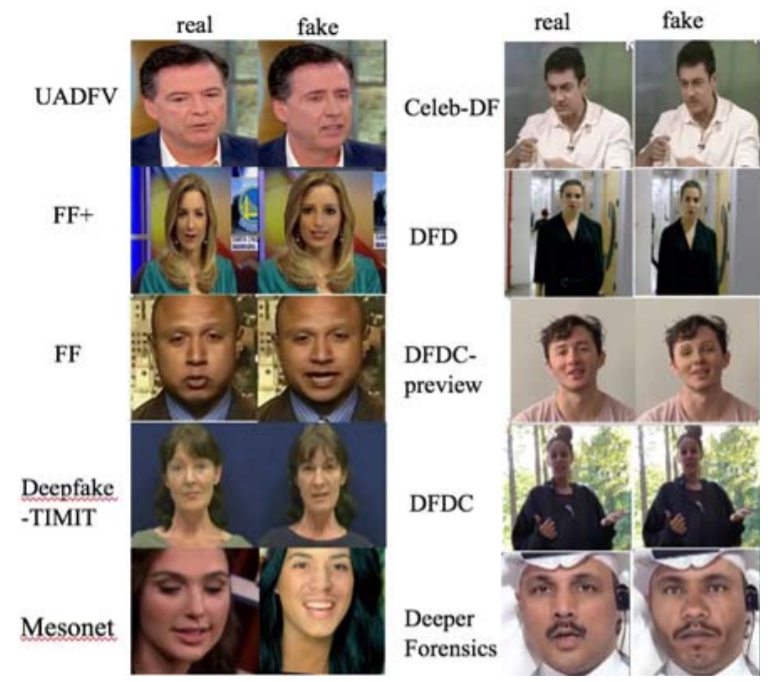
\includegraphics[width=0.60\textwidth]{img/ch2m1.png} 
\caption{Li XR 等人 \cite{2021496} 的工作总结的资料对比}
\label{Test}
\end{figure}
